
\documentclass[12pt]{article}


%%% PACKAGES

\usepackage[pdftex]{graphicx}

\usepackage{hyperref}
\usepackage{bibentry} %to use intext full bibliography entries instead of citations.  You will need a separate BibTex database for this to work.  See http://cst.usc.edu/services/tel/grants/legrants.html for details on this package.
\usepackage{booktabs} % for much better looking tables
\usepackage{array} % for better arrays (eg matrices) in maths
\usepackage{paralist} % very flexible & customisable lists (eg. enumerate/itemize, etc.)
%\usepackage{verbatim} % adds environment for commenting out blocks of text & for better verbatim
%\usepackage{subfigure} % make it possible to include more than one captioned figure/table in a single float

\usepackage{caption}

\usepackage{color}

%%% PAGE DIMENSIONS
\usepackage{geometry} % to change the page dimensions. Read ftp://ftp.tex.ac.uk/tex-archive/macros/latex/contrib/geometry/geometry.pdf for detailed page layout information 
\geometry{margin=1in} % for example, change the margins to 1 inches all round
%\geometry{landscape} % set up the page for landscape
% 

%%% HEADERS & FOOTERS
\usepackage{fancyhdr} % This should be set AFTER setting up the page geometry
\pagestyle{fancy} % options: empty , plain , fancy
\renewcommand{\headrulewidth}{0.4pt} % customise the layout...
%\lhead{}\chead{}\rhead{}
%\lfoot{}\cfoot{\thepage}\rfoot{}

%\rfoot{\footnotesize SIR 330}
\rhead{\footnotesize BME 3300 Lab 4: Microcontrollers}
\renewcommand\footrulewidth{0pt}

\usepackage{enumitem}
%%% SECTION TITLE APPEARANCE
%\usepackage{sectsty}
%\allsectionsfont{\sffamily\mdseries\upshape} % (See the fntguide.pdf for font help)
% (This matches ConTeXt defaults)


%% END Article customise

%%% BEGIN DOCUMENT


\begin{document}


\thispagestyle{plain} %alternatively specify empty to get no footer on first page.  This is part of the fancyhdr package


\nobibliography{MasterBib} %this specifies the BibTex directory that stores your desired bibliography entries.  It has to come before any \bibentry lines are invoked

\bibliographystyle{apalike} %be careful here, there is only a few styles that will run


%\tableofcontents
\begin{center}

\textbf{BME 3300 Lab 4: Microcontrollers} \medskip

\end{center}

\section*{Objective} The objective of this lab exercise is to become familiar and comfortable working with
microcontrollers, using the Arduino platform. 
Specifically, you will learn how to connect sensors to an Arduino and program it to process measurements
from those sensors. 
You will then program the Arduino to actuate something based on its measurements.
The skills you gain from this lab can be applied to your semester projects, and/or to your senior design projects.
In recent years a large proportion of BME senior design projects have been based on Arduino. 

\section*{Microcontroller Background}
\subsection*{Functionality and Architecture}
Microcontrollers are small embedded real-time computers with sensing and actuating capabilities
that can be programmed to acquire and process data from sensors, and respond to those measurements.
Microcontrollers are ubiquitous, not only in biomedical devices but in the broader world. 
Wikipedia has a nice intro at http://en.wikipedia.org/wiki/Microcontroller.
Read the introduction, `History' and `Embedded Design' sections of that article.
\par Arduino has recently become a very popular platform for developing microcontroller applications, because it allows the developer
to write programs in a simple language (Processing), and makes it easy to download and execute those
programs on the chip, and to connect the chip to the outside world to do something useful. 

\subsection*{Arduino Hardware}
The Arduino Uno boards you will use in this lab exercise are based on the ATmega16U2 chip (the big chip on the board). 
A detailed description of the boards is available at
http://arduino.cc/en/Main/arduinoBoardUno

\subsection*{Arduino Programming}
Before getting started, familiarize yourself with programming and use of Arduino by reading the tutorials at
http://arduino.cc/en/Tutorial/Foundations. 
Pay particular attention to the Basics and Microcontrollers sections. 
Also read the Variables and Functions sections under Programming Technique.
Additional information about implementing commands Arduino utilizes can be found at http://arduino.cc/en/Reference/HomePage.

\section*{Procedure}
\subsection*{Task 1: Turning on an LED}
To start you will familiarize yourself with the programming IDE and 
load and execute an example program that blinks an LED on the UNO board on and off once every second.\\[1em]
Steps:
\begin{enumerate}
\item Plug in your Uno to your PC using the provided USB cable.
\item Start the Arduino software. 
Using the menu, open the {\bf Blink} sketch under File $\rightarrow$ Examples $\rightarrow$ Basics $\rightarrow$ Blink. 
The \texttt{setup()} function at the beginning of the sketch is called once when the board is powered on or reset, 
and is responsible for activities such as setting pin modes or initializing libraries. 
In this sketch it is used to set pin 13, which is connected to the `L' LED on the Uno board, to output mode.
The \texttt{loop()} function below that is what is actually repeatedly executed 
forever until the board is powered down or reset. 
This function contains the meat of the sketch. 
It is where the microcontroller is commanded to switch the LED on or off, 
and to wait for 1 second between switching modes.
\item Upload and run the sketch by clicking the right arrow button at the top of the Sketch editor window. 
After a few seconds you should see the LED blink on and off. 
Try changing the delays between on and off states and verify that the blinking frequency changes. 
Note that you may need to change the COM port that the PC is using to communicate with the Arduino. 
You can do this under Tools $\rightarrow$ Port.
\end{enumerate}

\subsection*{Task 2: Reading an analog input and control a PWM output}

In this task, you will measure an analog input voltage, display it on the (computer) screen, 
and set an LED brightness based on the value.

\begin{enumerate}
\item Open the {\bf AnalogInOutSerial} sketch from File $\rightarrow$ Examples $\rightarrow$ Analog. 
This sketch specifies an input channel (A0) and an output channel (9) at the beginning. 
It also declares the sensor and output values. 
This is important because before Arduino can use a variable or constant, it must be declared to the coder with a term like \texttt{int} for a 32-bit integer or \texttt{float} for a floating-point value. 
In \texttt{setup()}, serial communication is initiated at 9600 bps. 
This will allow you to see output values in the terminal window later. 
In \texttt{loop()}, the value on A0 is read, 
scaled to an 8 bit number and output as an analog voltage on pin 9.
\item As described in the beginning of the sketch, place the potentiometer and LED on your breadboard, and wire them to the Arduino board with the jumper wires. 
Change the \texttt{delay} value at the end of the sketch to 1000. 
Upload and run the sketch. 
Then, open a ``Serial Monitor'' window from the Tools menu.
\item You should see 2 values, sensor and output, on the screen. 
The LED should be lit, and when the potentiometer is adjusted, the LED value and sensor value should change. 
The PWM (pulse width modification) output to the LED is a form of digital to analog conversion. 
An 8-bit digital value is converted to a square wave with a variable on-time. 
Attach your oscilloscope to the output of pin 9 and see how changing the potentiometer affects the signal. \\
{\bf What is the frequency of the PWM output?} \\ 
\bigskip \bigskip \bigskip \\ 
{\bf How does the changing square wave control the LED brightness?}\\
\bigskip \bigskip \bigskip \\
{\bf What would change if you used a different size of potentiometer?}\\
\bigskip \bigskip \bigskip
\item The voltage at A0 is represented as a 10-bit integer from 0 to 1023. 
Change the sketch so that the actual voltage is calculated and displayed in the terminal. 
You may need to use a \texttt{float} variable, since \texttt{int} is an integer will not display any decimal places. 
Save the sketch to your 3300 folder and show the TA.\\
{\bf What is the voltage resolution of the Arduino board?}\\
\bigskip \bigskip \bigskip
\end{enumerate}

%http://dlnmh9ip6v2uc.cloudfront.net/\\
%datasheets/Dev/Arduino/Shields/16x2\_LCD\_Shield\_Spec\_Rev\_1.1\_20130318.pdf. 
\subsection*{Task 3: LCD Display}
A microcontroller can be more useful if it can be monitored and adjusted without the need for a computer. 
An LCD screen can be attached to an Arduino to relay messages and allow for user input. 
Information about the LCD can be found at \url{http://osepp.com/wp-content/uploads/2013/07/SPLC780D_DS.pdf}.
This is a 4-bit parallel screen meaning, 
4 data lines transmit the code for each character simultaneously in two 4-bit nibbles. 
This LCD screen also includes 5 buttons which each send a unique voltage to input A0.

\begin{enumerate}
\item Remove the connections from the Arduino board and plug in the LCD module, {\it being careful not to bend any of the leads.} 
Open the HelloWorld sketch from File $\rightarrow$ Examples $\rightarrow$ LiquidCrystal. 
Change the \texttt{LiquidCrystal lcd} parameter to \texttt{(8,9,4,5,6,7)} to match the different pinout of the LCD screen as shown in its datasheet. 
Upload the sketch and the screen should display \texttt{``hello, world''}. 
\item Re-attach the potentiometer, but this time in A1 and update your code to match. 
Add the code from your last sketch that calculates the voltage from the pot. 
Instead of printing the values over serial, send them to the LCD screen with the \texttt{lcd.clear()}, 
\texttt{lcd.setCoursor()}, and \texttt{lcd.print()} commands. 
Change the PWM output pin to 3, as pin 9 is now used by the LCD screen. A quick Google search for examples using the LCD screen can be helpful here.
\item Now add a line to the code to display the signal on A0 using \texttt{analogRead} when a button is pushed. 
Record the value for each button. 
Add code that allows you to increment and decrement an on-screen counter based on up/down button pushes. 
Use the \texttt{if} and comparison (\texttt{> and <}) operators to implement something like:
\begin{center}
\texttt{if (button > 100 \&\& button < 150) counter ++;}\\
\end{center}
to increase the counter. 
Add another line to decrease the counter when the down button is pushed. Note that you will need to determine what value A0 reads in association with each button press.  This can be done using the analogRead() function and displaying the output on the LCD screen as you press each button.\\
{\bf How can you control how fast the buttons change values?}\\
\bigskip \bigskip \bigskip \\
{\bf Have the TA verify your working board before continuing.}\\
\bigskip \bigskip \bigskip
\end{enumerate}

\subsection*{Task 4: Temperature sensor}

An easy way to measure temperature is with a thermistor. 
Read up about them at\\
http://ww1.microchip.com/downloads/cn/AppNotes/cn\_00685b.pdf  
and pay attention to the ``Introduction'' and ``Resistance vs temperature mode'' sections. 
We will be using NTC thermistors with a nominal value of 100 k$\Omega$ at 25$^{\circ}$ C. 
The downside of thermistors is their non-linear resistance change with temperature. 
This can be partly overcome by operating in a narrow temperature range where the output is more linear. 
Read the ``Linearization solutions'' section. 
You will set up your circuit like in Figure 5a.
Notice in Figure 6 over what range linear measurements can be made.

\begin{center}
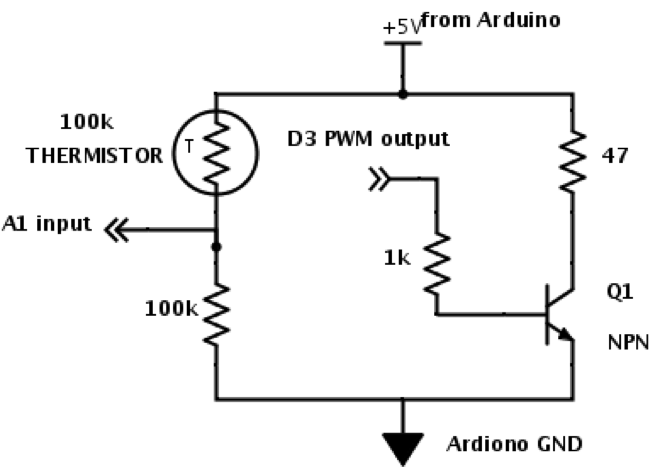
\includegraphics[width=0.5\textwidth,trim=0 0 0 0,clip=false]{thermistorcircuit.png}
\end{center}

\begin{enumerate}
\item Build the left half of the thermistor circuit shown above on the breadboard, 
using 5V power and GND from the Arduino board (you might have to pull the LCD off to see where the pins are). 
Attach the input to A1 on the board. 
The thermistor is the black, 4 lead device. 
It has a 47 $\Omega$ resistor attached to it for later use. 
The thermistor leads come out the bottom and the resistor leads out the sides. 
Use your last sketch to display the actual voltage from the thermistor.\\
{\bf How does this voltage change if you hold the thermistor with your fingers?}\\
\bigskip \bigskip \bigskip \\
\item Now you need to convert this voltage to an actual temperature. The following equation can be used for this calculation:
\[
	T = \frac{\beta}{\ln \left(\frac{R}{R_0e^{-\beta/T_0}}\right)},
\]
where $\beta$ is a thermistor property (3950 in this case), 
$R$ is the resistance at the given temperature (calculated from the voltage divider in the circuit above), 
$R_0$ is the nominal resistance (100 k$\Omega$) at $T_0$, and $T_0$ 
is room temperature (298 K). 
This equation yields temperature in Kelvin, so don't forget to convert to Celsius. 
Implement this equation in Arduino code. 
Use the LCD screen to troubleshoot your code and display the output.\\
{\bf What is the temperature resolution of your measurement?}\\
\bigskip \bigskip \bigskip \\
\end{enumerate}

\subsection*{Task 5: Temperature Control}

Imagine the thermistor/resistor package is really an incubator that you want kept at a certain temperature,
and the resistor is a heater. 
The simplest control method is to use a thermostat that turns the heater on when below the set point, and off when above the set point. 
However, this method can suffer from large swings in temperature as it cycles the heater on and off. 
Smoother temperature changes can be achieved using a 
Proportional Integral Derivative (PID) controller that can 
adjust the heater current in a continuous rather than binary manner, 
depending on the current measured temperature. 
You will implement a simple form of a Proportional Integral controller that 
sets the current based on the present and past temperature error. 
Microcontrollers are made for real-time applications like this since 
they can be set to run indefinitely with little or no outside control. 

\par You will program the Arduino to control the current going through 
the 47 $\Omega$ resistor to keep the thermistor at a set temperature. 
The resistor cannot be attached directly to the Arduino because the outputs only 
provide about 20 mA, which is not enough to create heating. 
However, this is plenty of current for driving a transistor. 
Transistors are key to every integrated circuit and function as a voltage or current amplifier, 
where a small signal controls a much larger one. 
You will use a 2N3904 transistor to control the current going to the resistor.

\begin{enumerate}
\item Build the right-hand side of the thermistor circuit shown above. 
Attach digital pin 3 to the transistor. 
Add \texttt{analogWrite} to your previous sketch and set the PWM output to 200 and view the transistor output on your oscilloscope. 
Verify operation further by monitoring the thermistor temperature as it rises.
\item Now you need to write a code that adjusts the heater output to achieve a steady temperature of 37$^{\circ}$ C. 
To do this, create a PWM and add or subtract from it according to the error between your set and actual temperature. 
The following equation is a very simplistic, modified Proportional Integral controller:
\[
	PWM = PWM_{prior} + P \cdot T_{error}.
\]
The $PWM_{prior}$ term acts as an integral because it represents the prior best guess output, which depends on the previous error and the error before that, and so on. 
$P$ is the proportional gain term. 
Put this equation in loop so that it updates and adjusts every iteration. 
Adjust $P$ so that the controller responds quickly to changes, 
but not so much that it becomes unstable and oscillates. 
The \texttt{constrain} function is useful to limit $PWM$ to 0-255 so as not to upset the Arduino. 
Display your set and actual temperature on the screen:
\begin{center}
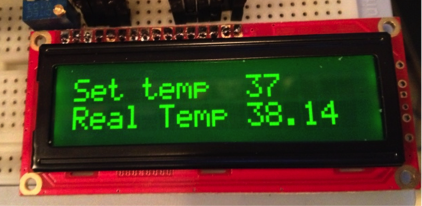
\includegraphics[width=0.5\textwidth,trim=0 0 0 0,clip=false]{screentemp.png}
\end{center}
\item Now incorporate code that will allow the buttons to change the temperature set point. 
See how the circuit responds to changes in the set point and adjust $P$ as necessary.\\
{\bf What is a good value for $P$?}\\
\bigskip \bigskip \bigskip \\
{\bf What else could be done to improve the accuracy and response of your controller?
Try implementing a real PI equation where the gain on the integral of the error can be adjusted:}
\[
	PWM = P\cdot T_{error} + I\cdot \sum T_{error}.
\]
\end{enumerate}

Congratulations, you can now build and program microcontrollers 
to interface with the world around you and control it!
{\bf Show the TA your completed device, then clean up your station and disassemble your Arduino board.}\\

\bigskip
\noindent Parts List:\\[0.4em]
\begin{tabular}{|l|c|}
\hline
Arduino Uno & 1 \\ \hline
USB Cable & 1 \\ \hline
LCD Screen & 1 \\ \hline
10 k$\Omega$ Potentiometer & 1 \\ \hline
Red LED & 1 \\ \hline
100 k$\Omega$ resistor & 2 \\ \hline
1 k$\Omega$ resistor & 2 \\ \hline
NTC 100k$\Omega$ @ 25$^{\circ}$ thermistor package & 1 \\ \hline
NPN Transistor & 1 \\ \hline
Breadboard & 1 \\ \hline
Jumper Wires & 10 \\ \hline
\end{tabular}


\end{document} 